\begin{pastexam}[label={px:ncku-111-cce-ds-03}]{成大電通所 111 學年度 第 3 題}
（問答）

(10 \textbf{pts}) Tree
\begin{enumerate}[label=\alph*.]
\item (5 \textbf{pts}) Consider the following Huffman coding table:\\
\hspace*{3em}A: 11, B:10, C:001, D: 000, E:01\\
Please decode the string ``10001110111000'' into the source string (note that you have to draw
your Huffman code tree first).
\item (5 \textbf{pts}) Draw the threaded representation of the resulting binary tree in (a) if you
want to traverse the graph in pre-order traverse? Note that you nedd use solid line to point to
the predecessor of a node and a dash line to point to the successor of a node.
\end{enumerate}
\end{pastexam}

\begin{pastsoln}
答案：(a) BCAEAD；(b) 見下面的引線樹。 (a) 和資結書第~19.3~節的霍夫曼編碼有關，但題目只是用碼表
建樹、解碼；(b) 是第~7.5~節的引線二元樹，本題放在第~7~章。

\textbf{(a) 建樹。} 每個碼字從根走下去，0 往左、1 往右，走完的位置放那個字元。 五個碼字
$11, 10, 001, 000, 01$ 沒有一個是另一個的前綴（prefix code），所以字元都在葉節點上。 內部節點
依前序取名 $r, p, q, s$：
\begin{center}
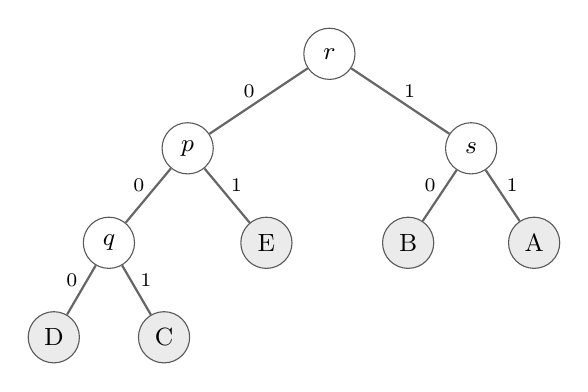
\begin{tikzpicture}[
    btn/.style={circle, draw=black!65, line width=0.4pt, minimum size=6.5mm, inner sep=0pt, font=\small},
    lf/.style={btn, fill=black!8},
    e/.style={draw=black!60, thick}, lab/.style={font=\scriptsize, inner sep=1pt}]
\node[btn] (r) at (0,0) {$r$};
\node[btn] (p) at (-1.8,-1.2) {$p$};
\node[btn] (s) at (1.8,-1.2) {$s$};
\node[btn] (q) at (-2.8,-2.4) {$q$};
\node[lf] (E) at (-0.8,-2.4) {E};
\node[lf] (B) at (1.0,-2.4) {B};
\node[lf] (A) at (2.6,-2.4) {A};
\node[lf] (D) at (-3.5,-3.6) {D};
\node[lf] (C) at (-2.1,-3.6) {C};
\draw[e] (r) -- node[lab,above left] {0} (p);
\draw[e] (r) -- node[lab,above right] {1} (s);
\draw[e] (p) -- node[lab,above left] {0} (q);
\draw[e] (p) -- node[lab,above right] {1} (E);
\draw[e] (s) -- node[lab,above left] {0} (B);
\draw[e] (s) -- node[lab,above right] {1} (A);
\draw[e] (q) -- node[lab,above left] {0} (D);
\draw[e] (q) -- node[lab,above right] {1} (C);
\end{tikzpicture}
\end{center}

\textbf{解碼。} 從根開始照位元往下走，碰到葉節點就輸出那個字元、回到根：
\begin{center}
\begin{tabular}{ccc}
\toprule
讀到的位元 & 走的路徑 & 輸出 \\
\midrule
1 0 & $r \to s \to$ B & B \\
0 0 1 & $r \to p \to q \to$ C & C \\
1 1 & $r \to s \to$ A & A \\
0 1 & $r \to p \to$ E & E \\
1 1 & $r \to s \to$ A & A \\
0 0 0 & $r \to p \to q \to$ D & D \\
\bottomrule
\end{tabular}
\end{center}
$2 + 3 + 2 + 2 + 2 + 3 = 14$ 個位元剛好用完，原字串是 \textbf{BCAEAD}。

\textbf{(b) 前序引線樹。} 把每個空的指標換成引線（資結書第~7.5~節）：題目要的是前序走訪，所以
空的\textbf{左}指標指向\textbf{前序的前一個}（predecessor，實線），空的\textbf{右}指標指向
\textbf{前序的下一個}（successor，虛線）。 前序是
\[
r,\ p,\ q,\ \mathrm{D},\ \mathrm{C},\ \mathrm{E},\ s,\ \mathrm{B},\ \mathrm{A}.
\]
霍夫曼樹的內部節點都有兩個孩子，空指標只在五個葉節點上，共 $2 \times 5 = 10$ 條引線（$n = 9$
個節點，空指標 $n + 1 = 10$ 個，對得上）：
\begin{center}
\begin{tabular}{lll}
\toprule
節點 & 左引線（實線，前一個） & 右引線（虛線，下一個） \\
\midrule
D & $q$ & C \\
C & D & E \\
E & C & $s$ \\
B & $s$ & A \\
A & B & 無（\NIL；有頭節點的話指向頭節點） \\
\bottomrule
\end{tabular}
\end{center}
下圖細灰線是原本的樹邊，箭頭是引線：
\begin{center}
\begin{tikzpicture}[>={Stealth[length=2mm]},
    btn/.style={circle, draw=black!65, line width=0.4pt, minimum size=6.5mm, inner sep=0pt, font=\small},
    lf/.style={btn, fill=black!8},
    e/.style={draw=black!35, thin},
    pred/.style={->, thick}, succ/.style={->, thick, dashed}]
\node[btn] (r) at (0,0) {$r$};
\node[btn] (p) at (-2.2,-1.3) {$p$};
\node[btn] (s) at (2.2,-1.3) {$s$};
\node[btn] (q) at (-3.4,-2.7) {$q$};
\node[lf] (E) at (-1.0,-2.7) {E};
\node[lf] (B) at (1.2,-2.9) {B};
\node[lf] (A) at (3.3,-2.9) {A};
\node[lf] (D) at (-4.3,-4.3) {D};
\node[lf] (C) at (-2.4,-4.3) {C};
\draw[e] (r) -- (p); \draw[e] (r) -- (s);
\draw[e] (p) -- (q); \draw[e] (p) -- (E);
\draw[e] (s) -- (B); \draw[e] (s) -- (A);
\draw[e] (q) -- (D); \draw[e] (q) -- (C);
% 左引線（實線）：指向前序的前一個
\draw[pred] (D.north west) to[bend left=40] (q.west);
\draw[pred] (C.south west) to[bend left=35] (D.south east);
\draw[pred] (E.south) to[bend left=25] (C.east);
\draw[pred] (B.north west) to[bend left=30] (s.west);
\draw[pred] (A.south west) to[bend left=30] (B.south east);
% 右引線（虛線）：指向前序的下一個
\draw[succ] (D.east) to[bend left=30] (C.west);
\draw[succ] (C.north east) to[bend right=25] (E.south west);
\draw[succ] (E.east) to[bend right=20] (s.south west);
\draw[succ] (B.east) to[bend left=30] (A.west);
\draw[succ] (A.east) -- ++(0.8,0) node[right, font=\small] {\NIL};
\end{tikzpicture}
\end{center}
用引線做前序走訪：在節點 $x$ 時，有左孩子就往左；沒有左孩子（左邊是引線）而有右孩子就往右；
兩邊都是引線就沿右引線走。 從 $r$ 出發依序得到 $r, p, q,$ D, C, E, $s,$ B, A，A 的右引線是
\NIL，結束。 實際存放時每個指標旁邊還要一個標記位元（$\mathit{leftThread}$、
$\mathit{rightThread}$），分辨它是孩子還是引線。
\end{pastsoln}
